% WTune structure map (src/wtune at 1011f32): CLI -> five stages -> modules -> site/launcher.
% Build: pdflatex wtune-structure.tex
\documentclass[tikz,border=10pt]{standalone}
\usepackage[T1]{fontenc}
\usepackage{lmodern}
\usetikzlibrary{positioning,fit,arrows.meta,backgrounds,calc}

\definecolor{cli}{HTML}{37474F}
\definecolor{setup}{HTML}{5E35B1}
\definecolor{prep}{HTML}{00897B}
\definecolor{tune}{HTML}{1E88E5}
\definecolor{run}{HTML}{E64A19}
\definecolor{post}{HTML}{2E7D32}
\definecolor{site}{HTML}{6D4C41}
\definecolor{shared}{HTML}{616161}

\tikzset{
  m/.style={draw=#1, fill=#1!8, rounded corners=2pt, font=\scriptsize\ttfamily,
            align=center, inner sep=3pt, minimum height=7mm, text width=#1w},
  box/.style 2 args={draw=#1, fill=#1!8, rounded corners=2pt, font=\scriptsize\ttfamily,
            align=center, inner sep=3pt, minimum height=7mm, text width=#2},
  cmd/.style={draw=#1, fill=#1!22, rounded corners=3pt, font=\small\bfseries\ttfamily,
              minimum height=7mm, inner sep=4pt, align=center},
  head/.style={draw=#1, fill=#1!22, rounded corners=3pt, font=\footnotesize\bfseries,
               text=#1!70!black, inner sep=3pt, align=center},
  grp/.style={draw=#1, thick, rounded corners=6pt, inner sep=5pt, fill=#1!3},
  flow/.style={-{Stealth[length=2.2mm]}, thick, draw=#1},
  data/.style={-{Stealth[length=1.8mm]}, densely dashed, draw=black!55},
  file/.style={draw=black!50, fill=yellow!14, font=\scriptsize\ttfamily, inner sep=3pt,
               align=center},
  lbl/.style={font=\tiny\itshape, fill=white, inner sep=1pt},
}

\begin{document}
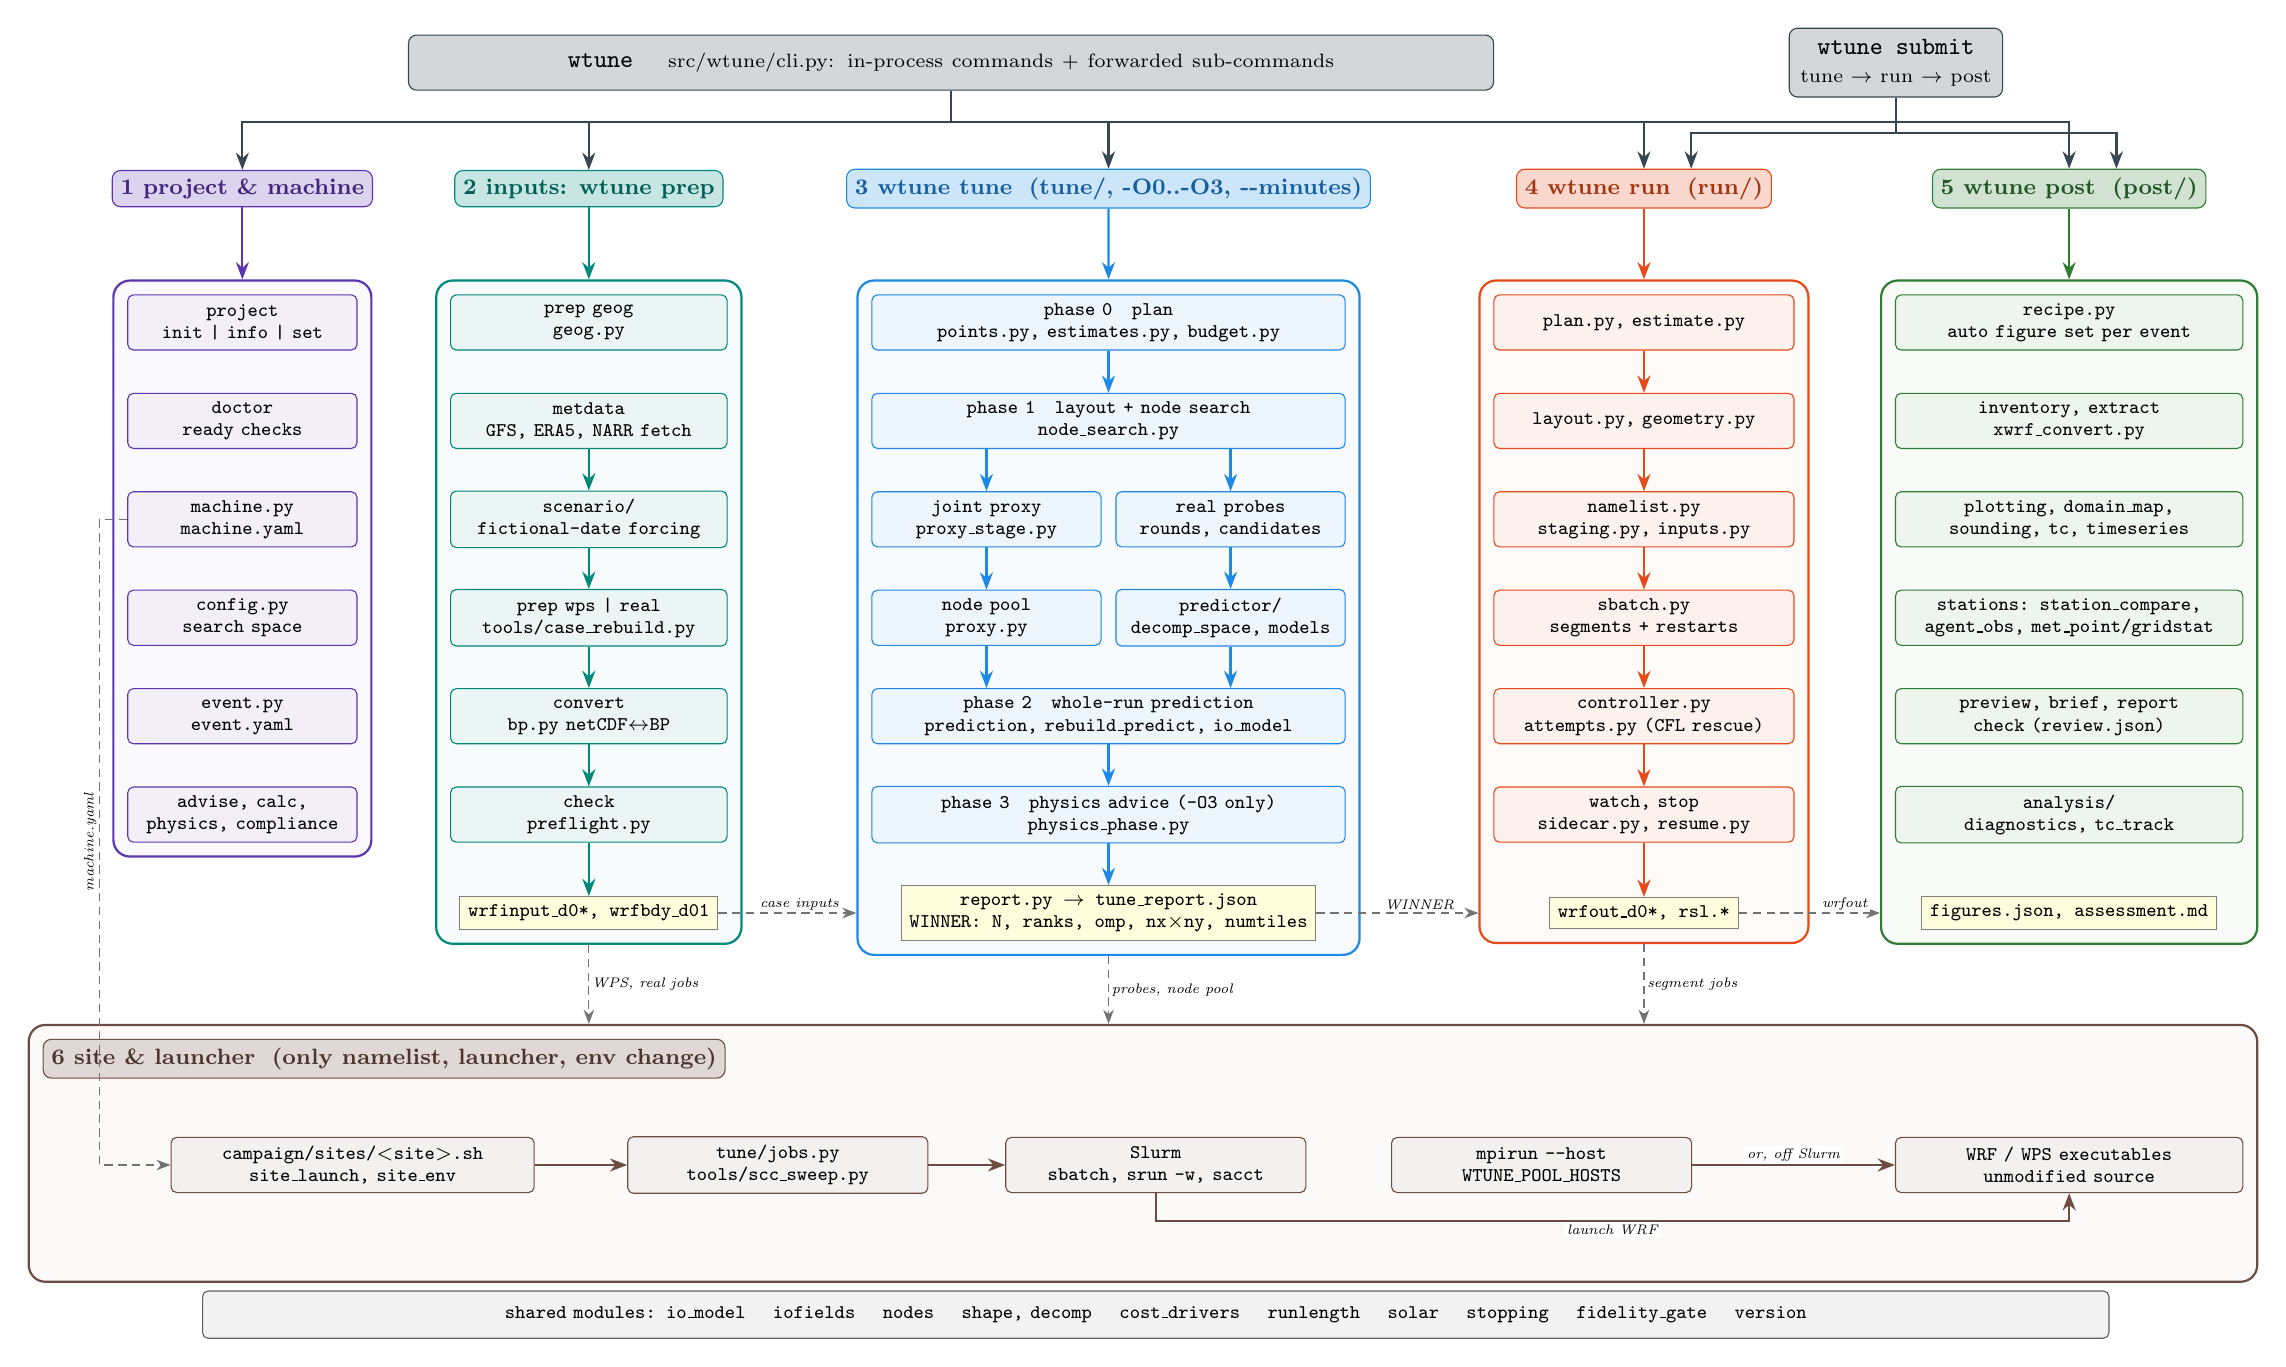
\begin{tikzpicture}

% column centres and row pitch
\def\xA{0}\def\xB{4.4}\def\xC{11.0}\def\xD{17.8}\def\xE{23.2}
\def\dy{1.25}

% ---------------- entry ----------------
\node[cmd=cli, text width=13.5cm] (cli) at (9.0,3.3)
  {wtune \quad\normalfont\scriptsize src/wtune/cli.py: in-process commands + forwarded sub-commands};
\node[cmd=cli] (submit) at (21.0,3.3) {wtune submit\\[-1pt]\normalfont\scriptsize tune $\to$ run $\to$ post};

% ---------------- headers ----------------
\node[head=setup] (h1) at (\xA,1.7) {1 project \& machine};
\node[head=prep]  (h2) at (\xB,1.7) {2 inputs: wtune prep};
\node[head=tune]  (h3) at (\xC,1.7) {3 wtune tune \;(tune/, -O0..-O3, -{}-minutes)};
\node[head=run]   (h4) at (\xD,1.7) {4 wtune run \;(run/)};
\node[head=post]  (h5) at (\xE,1.7) {5 wtune post \;(post/)};

\coordinate (bus) at (0,2.55);
\foreach \h in {h1,h2,h3,h4,h5} {
  \draw[flow=cli] (cli.south) |- (\h.north |- bus) -- (\h.north);
}
\draw[flow=cli] (submit.south) -- ++(0,-0.45) -| ($(h4.north)+(0.6,0)$);
\draw[flow=cli] (submit.south) -- ++(0,-0.45) -| ($(h5.north)+(0.6,0)$);

% ---------------- 1 setup ----------------
\node[box={setup}{27mm}] (project) at (\xA,0) {project\\init | info | set};
\node[box={setup}{27mm}] (doctor) at (\xA,-\dy) {doctor\\ready checks};
\node[box={setup}{27mm}] (machine) at (\xA,-2*\dy) {machine.py\\machine.yaml};
\node[box={setup}{27mm}] (config) at (\xA,-3*\dy) {config.py\\search space};
\node[box={setup}{27mm}] (event) at (\xA,-4*\dy) {event.py\\event.yaml};
\node[box={setup}{27mm}] (advise) at (\xA,-5*\dy) {advise, calc,\\physics, compliance};
\begin{scope}[on background layer]
  \node[grp=setup, fit=(project)(advise)] (g1) {};
\end{scope}
\draw[flow=setup] (h1) -- (g1.north);

% ---------------- 2 prep ----------------
\node[box={prep}{33mm}] (geog) at (\xB,0) {prep geog\\geog.py};
\node[box={prep}{33mm}] (metdata) at (\xB,-\dy) {metdata\\GFS, ERA5, NARR fetch};
\node[box={prep}{33mm}] (scen) at (\xB,-2*\dy) {scenario/\\fictional-date forcing};
\node[box={prep}{33mm}] (wps) at (\xB,-3*\dy) {prep wps | real\\tools/case\_rebuild.py};
\node[box={prep}{33mm}] (bp) at (\xB,-4*\dy) {convert\\bp.py netCDF$\leftrightarrow$BP};
\node[box={prep}{33mm}] (pre) at (\xB,-5*\dy) {check\\preflight.py};
\node[file] (inp) at (\xB,-6*\dy) {wrfinput\_d0*, wrfbdy\_d01};
\begin{scope}[on background layer]
  \node[grp=prep, fit=(geog)(inp)] (g2) {};
\end{scope}
\draw[flow=prep] (h2) -- (g2.north);
\draw[flow=prep] (metdata) -- (scen); \draw[flow=prep] (scen) -- (wps);
\draw[flow=prep] (wps) -- (bp); \draw[flow=prep] (bp) -- (pre); \draw[flow=prep] (pre) -- (inp);

% ---------------- 3 tune ----------------
\node[box={tune}{58mm}] (p0) at (\xC,0) {phase 0 \; plan\\points.py, estimates.py, budget.py};
\node[box={tune}{58mm}] (p1) at (\xC,-\dy) {phase 1 \; layout + node search\\node\_search.py};
\node[box={tune}{27mm}] (joint) at (\xC-1.55,-2*\dy) {joint proxy\\proxy\_stage.py};
\node[box={tune}{27mm}] (real) at (\xC+1.55,-2*\dy) {real probes\\rounds, candidates};
\node[box={tune}{27mm}] (pool) at (\xC-1.55,-3*\dy) {node pool\\proxy.py};
\node[box={tune}{27mm}] (pred) at (\xC+1.55,-3*\dy) {predictor/\\decomp\_space, models};
\node[box={tune}{58mm}] (p2) at (\xC,-4*\dy) {phase 2 \; whole-run prediction\\prediction, rebuild\_predict, io\_model};
\node[box={tune}{58mm}] (p3) at (\xC,-5*\dy) {phase 3 \; physics advice (-O3 only)\\physics\_phase.py};
\node[file] (trep) at (\xC,-6*\dy) {report.py $\to$ tune\_report.json\\WINNER: N, ranks, omp, nx$\times$ny, numtiles};
\begin{scope}[on background layer]
  \node[grp=tune, fit=(p0)(joint)(real)(trep)] (g3) {};
\end{scope}
\draw[flow=tune] (h3) -- (g3.north);
\draw[flow=tune] (p0) -- (p1);
\draw[flow=tune] (p1.south -| joint) -- (joint);
\draw[flow=tune] (p1.south -| real) -- (real);
\draw[flow=tune] (joint) -- (pool);
\draw[flow=tune] (real) -- (pred);
\draw[flow=tune] (pool) -- (p2.north -| pool);
\draw[flow=tune] (pred) -- (p2.north -| pred);
\draw[flow=tune] (p2) -- (p3);
\draw[flow=tune] (p3) -- (trep);

% ---------------- 4 run ----------------
\node[box={run}{36mm}] (rplan) at (\xD,0) {plan.py, estimate.py};
\node[box={run}{36mm}] (rlay) at (\xD,-\dy) {layout.py, geometry.py};
\node[box={run}{36mm}] (rnl) at (\xD,-2*\dy) {namelist.py\\staging.py, inputs.py};
\node[box={run}{36mm}] (rsb) at (\xD,-3*\dy) {sbatch.py\\segments + restarts};
\node[box={run}{36mm}] (rctl) at (\xD,-4*\dy) {controller.py\\attempts.py (CFL rescue)};
\node[box={run}{36mm}] (rwatch) at (\xD,-5*\dy) {watch, stop\\sidecar.py, resume.py};
\node[file] (wrfout) at (\xD,-6*\dy) {wrfout\_d0*, rsl.*};
\begin{scope}[on background layer]
  \node[grp=run, fit=(rplan)(wrfout)] (g4) {};
\end{scope}
\draw[flow=run] (h4) -- (g4.north);
\foreach \a/\b in {rplan/rlay, rlay/rnl, rnl/rsb, rsb/rctl, rctl/rwatch, rwatch/wrfout}
  \draw[flow=run] (\a) -- (\b);

% ---------------- 5 post ----------------
\node[box={post}{42mm}] (recipe) at (\xE,0) {recipe.py\\auto figure set per event};
\node[box={post}{42mm}] (extract) at (\xE,-\dy) {inventory, extract\\xwrf\_convert.py};
\node[box={post}{42mm}] (plots) at (\xE,-2*\dy) {plotting, domain\_map,\\sounding, tc, timeseries};
\node[box={post}{42mm}] (obs) at (\xE,-3*\dy) {stations: station\_compare,\\agent\_obs, met\_point/gridstat};
\node[box={post}{42mm}] (review) at (\xE,-4*\dy) {preview, brief, report\\check (review.json)};
\node[box={post}{42mm}] (ana) at (\xE,-5*\dy) {analysis/\\diagnostics, tc\_track};
\node[file] (figs) at (\xE,-6*\dy) {figures.json, assessment.md};
\begin{scope}[on background layer]
  \node[grp=post, fit=(recipe)(figs)] (g5) {};
\end{scope}
\draw[flow=post] (h5) -- (g5.north);

% ---------------- data hand-offs ----------------
\draw[data] (inp.east) -- (inp.east -| g3.west);
\path (inp.east -| g2.east) -- node[lbl, above]{case inputs} (inp.east -| g3.west);
\draw[data] (trep.east) -- (trep.east -| g4.west);
\path (trep.east -| g3.east) -- node[lbl, above]{WINNER} (trep.east -| g4.west);
\draw[data] (wrfout.east) -- (wrfout.east -| g5.west);
\path (wrfout.east -| g4.east) -- node[lbl, above]{wrfout} (wrfout.east -| g5.west);

% ---------------- 6 site layer ----------------
\def\ys{-10.7}
\node[head=site] (h6) at (\xA+1.8,\ys+1.35) {6 site \& launcher \;(only namelist, launcher, env change)};
\node[box={site}{44mm}] (sites) at (\xA+1.4,\ys) {campaign/sites/\textless site\textgreater.sh\\site\_launch, site\_env};
\node[box={site}{36mm}] (jobs) at (\xB+2.4,\ys) {tune/jobs.py\\tools/scc\_sweep.py};
\node[box={site}{36mm}] (slurm) at (\xC+0.6,\ys) {Slurm\\sbatch, srun -w, sacct};
\node[box={site}{36mm}] (mpi) at (\xD-1.3,\ys) {mpirun --host\\WTUNE\_POOL\_HOSTS};
\node[box={site}{42mm}] (wrf) at (\xE,\ys) {WRF / WPS executables\\unmodified source};
\coordinate (g6low) at ($(slurm.south)+(0,-0.95)$);
\begin{scope}[on background layer]
  \node[grp=site, fit=(h6)(sites)(wrf)(g6low)] (g6) {};
\end{scope}
\draw[flow=site] (sites) -- (jobs);
\draw[flow=site] (jobs) -- (slurm);
\draw[flow=site] (slurm.south) -- ++(0,-0.35) -| node[lbl, pos=0.25, below]{launch WRF} (wrf.south);
\draw[flow=site] (mpi) -- node[lbl, above]{or, off Slurm} (wrf);

% jobs leave every stage through the site layer
\draw[data] (machine.west) -- ++(-0.35,0) |- node[lbl, pos=0.25, rotate=90, above]{machine.yaml} (sites.west);
\draw[data] (g2.south) -- node[lbl, right]{WPS, real jobs} (g2.south |- g6.north);
\draw[data] (g3.south) -- node[lbl, right]{probes, node pool} (g3.south |- g6.north);
\draw[data] (g4.south) -- node[lbl, right]{segment jobs} (g4.south |- g6.north);

% ---------------- shared ----------------
\node[box={shared}{240mm}, minimum height=6mm] (sharedm) at (11.6,\ys-1.9)
  {shared modules: io\_model \quad iofields \quad nodes \quad shape, decomp \quad cost\_drivers \quad runlength \quad solar \quad stopping \quad fidelity\_gate \quad version};

\end{tikzpicture}
\end{document}
